\section{Análise Comparativa Global: Métodos Diretos versus Iterativos}

A formulação de soluções para sistemas lineares da forma $Ax = b$ repousa sobre dois paradigmas fundamentais da análise numérica: a manipulação algébrica em passos finitos e a convergência assintótica por relaxação. A priori, a escolha empírica entre métodos diretos (Eliminação de Gauss, Fatoração LU, Gauss-Jordan) e iterativos (Gauss-Jacobi, Gauss-Seidel) transcende a mera obtenção do vetor resposta, englobando uma avaliação rigorosa do custo computacional, da topologia matricial (esparsidade) e da sensibilidade aos erros de máquina subjacentes à arquitetura de ponto flutuante.

\subsection{Exatidão Algébrica e Esforço Computacional Base}

Os métodos diretos fundamentam-se em transformações topológicas contíguas que, na ausência de erros de arredondamento, garantiriam a solução analítica exata. A Eliminação de Gauss e suas variantes operam sob uma complexidade de tempo assintótica dominada por $\mathcal{O}(n^3)$ operações de ponto flutuante (flops). Por outro lado, os métodos iterativos abdicam da exatidão formal imediata em prol da construção de uma sequência de vetores $\{x^{(k)}\}$ regida por uma tolerância de convergência $\epsilon$. O custo por iteração cai drasticamente para $\mathcal{O}(n^2)$ (ou até $\mathcal{O}(n)$ em malhas altamente esparsas). No entanto, a viabilidade dessa abordagem depende intrinsecamente do raio espectral da matriz de iteração, exigindo que as propriedades de dominância diagonal sejam estritamente atendidas para evitar a divergência irrestrita.

\subsection{Avaliação de Desempenho Numérico e Custo de Fases}

A fim de quantificar os paralelos conceituais, a Tabela \ref{tab:comparativo_52} consolida o embate entre as vertentes aplicado ao balanceamento elétrico do Problema Teste 5.2. O sistema em questão apresentou condicionamento favorável e simetria contínua.

\begin{table}[H]
\centering
\caption{Desempenho Global na Resolução do Circuito (Problema 5.2)}
\label{tab:comparativo_52}
\resizebox{\textwidth}{!}{%
\begin{tabular}{lccc}
\hline
\textbf{Classe do Método} & \textbf{Algoritmo Específico} & \textbf{Passos / Iterações} & \textbf{Vetor Solução $x^* \approx [i_1, i_2, i_3]^T$} \\ \hline
Direto & Eliminação de Gauss & 7 & $[2.0000, 1.0000, 1.0000]^T$ \\
Direto & Gauss-Jordan & 10 & $[2.0000, 1.0000, 1.0000]^T$ \\
Direto & Fatoração LU & 13 & $[2.0000, 1.0000, 1.0000]^T$ \\ \hline
Iterativo & Gauss-Jacobi & 8 & $[1.9747, 0.9783, 0.9824]^T$ \\
Iterativo & Gauss-Seidel & 6 & $[1.9949, 0.9970, 0.9982]^T$ \\ \hline
\end{tabular}%
}
\end{table}

A análise crítica dos resultados evidencia que os métodos diretos atingiram a solução exata ancorada no limite do ruído de máquina, extraindo a raiz inteira $(2, 1, 1)$. Entre eles, a Eliminação de Gauss provou-se a mais econômica, consumindo apenas 7 etapas macro de processamento frente às 10 de Jordan, visto que este último penaliza o tempo de CPU ao exigir a anulação de hiperplanos superiores e inferiores simultaneamente. Observa-se ainda que, embora a Fatoração LU tenha requerido 13 estágios sistêmicos, esse custo adicional configura um investimento estrutural: a matriz fatorada permite resoluções subsequentes em $\mathcal{O}(n^2)$ caso o vetor de restrição elétrica $b$ venha a flutuar iterativamente.

No espectro iterativo, submetidos a uma restrição de erro relativo $< 10^{-2}$, as aproximações pararam nas vizinhanças do vetor ideal. Gauss-Seidel necessitou de apenas 6 iterações para superar a precisão de Gauss-Jacobi (que demandou 8). Essa diferença corrobora a tese de que a atualização instantânea do passo algorítmico potencializa o atrito numérico rumo à origem do plano dimensional.

\subsection{Comportamento Iterativo em Matrizes Esparsas}

Quando as dimensões da matriz escalonam, o comportamento algorítmico se bifurca. Os métodos diretos demonstram uma falha catastrófica conhecida como fenômeno de preenchimento (\textit{fill-in}) em malhas de equações diferenciais, onde a alocação de multiplicadores aniquila a esparsidade, consumindo memória restritiva. Para contornar essa falha, os métodos iterativos dominam integralmente a resolução de modelos como o de Laplace (Problema 5.1) e da Difusão Térmica (Problema 5.5).

Durante as iterações na malha $6 \times 6$ de Laplace, sob um limiar de exatidão $\epsilon < 10^{-4}$, Gauss-Jacobi exigiu 17 iterações, enquanto Gauss-Seidel convergiu em apenas 10. Torna-se ainda mais evidente a escalabilidade deste fenômeno ao analisar a malha térmica $9 \times 9$:

\begin{figure}[H]
\centering
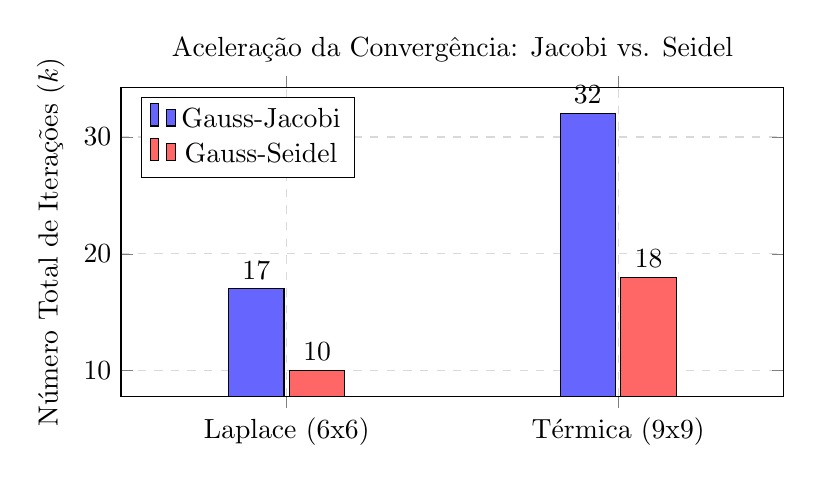
\begin{tikzpicture}
\begin{axis}[
    width=10cm, height=5.5cm,
    ybar,
    bar width=20pt,
    enlarge x limits=0.5,
    ylabel={Número Total de Iterações ($k$)},
    symbolic x coords={Laplace (6x6), Térmica (9x9)},
    xtick=data,
    nodes near coords,
    nodes near coords align={vertical},
    grid=major,
    grid style={dashed, gray!30},
    title={Aceleração da Convergência: Jacobi vs. Seidel},
    legend pos=north west
]
\addplot[fill=blue!60] coordinates {(Laplace (6x6),17) (Térmica (9x9),32)};
\addplot[fill=red!60] coordinates {(Laplace (6x6),10) (Térmica (9x9),18)};
\legend{Gauss-Jacobi, Gauss-Seidel}
\end{axis}
\end{tikzpicture}
\caption{Aceleração da Convergência: Jacobi vs. Seidel}
\label{fig:comparacao_aceleracao}
\end{figure}

A relação causal para essa disparidade repousa na quebra de inércia da propagação de dados. Por mais que ambos os métodos convirjam em sistemas diagonalmente dominantes, Gauss-Seidel utiliza os valores recém-computados $x_i^{(k+1)}$ no exato instante em que interage com $x_{i+1}^{(k)}$. Em matrizes esparsas derivadas de EDPs, esse arranjo simula o fluxo físico contínuo de calor ou potencial com maior aderência temporal, reduzindo praticamente pela metade o acúmulo de processamento flutuante da Unidade Lógica Aritmética (ALU).

\subsection{Sensibilidade, Condicionamento e Robustez}

Uma avaliação comparativa profunda impõe que se discuta a robustez estrutural das rotinas frente ao condicionamento. Os métodos diretos são consideravelmente menos dependentes de restrições topológicas estritas. Caso a matriz possua zeros na diagonal principal, a adoção da heurística de pivotamento parcial resguarda os métodos exatos, estabilizando os multiplicadores sem perdas severas. Em contrapartida, os métodos iterativos não admitem a reestruturação in-loco (pois isso destruiria a arquitetura de banda ou a diagonalidade) e falham abruptamente, divergindo ao infinito caso a premissa do raio espectral favorável não se sustente.

Adicionalmente, os diretos não requerem "chute inicial" vetorial nem heurística para escolha de tolerância. Eles entregam a capacidade máxima que a aritmética de máquina suporta. Já os métodos iterativos exigem uma engenharia fina na determinação do erro aceitável e da semente $x_0$, a qual, se mal postulada, pode introduzir dezenas de ciclos ociosos na malha térmica antes que a perturbação atinja a fronteira de relaxação.

\subsection{Conclusão da Avaliação Sistêmica}

A síntese empírica e analítica dos testes consolidados dita um limite preclaro para a adoção computacional. Observa-se que métodos diretos (com protagonismo de Gauss e LU) estabelecem-se como a arquitetura mandatória para matrizes densas de pequeno e médio porte, fornecendo a confiabilidade máxima perante sistemas onde se exige o retorno exato estrito. A Fatoração LU evidencia-se soberana quando o preceito analítico demandar a reutilização dinâmica de $b$. 

Por outro lado, em sistemas esparsos e de ordem vastamente dilatada — inerentes a malhas de diferenças finitas tridimensionais ou redes de interconexão massiva — os métodos iterativos assumem o protagonismo numérico absoluto. Dessa forma, as aproximações assintóticas transmutam a limitação de precisão em uma vantagem insuperável de tempo e eficiência em memória espacial. Entre eles, Gauss-Seidel consagra-se pragmaticamente superior a Gauss-Jacobi, abatendo o custo computacional por ciclo iterativo sem comprometer o vetor solução projetado.